\documentclass[man]{apa6}
\usepackage{lmodern}
\usepackage{amssymb,amsmath}
\usepackage{ifxetex,ifluatex}
\usepackage{fixltx2e} % provides \textsubscript
\ifnum 0\ifxetex 1\fi\ifluatex 1\fi=0 % if pdftex
  \usepackage[T1]{fontenc}
  \usepackage[utf8]{inputenc}
\else % if luatex or xelatex
  \ifxetex
    \usepackage{mathspec}
  \else
    \usepackage{fontspec}
  \fi
  \defaultfontfeatures{Ligatures=TeX,Scale=MatchLowercase}
\fi
% use upquote if available, for straight quotes in verbatim environments
\IfFileExists{upquote.sty}{\usepackage{upquote}}{}
% use microtype if available
\IfFileExists{microtype.sty}{%
\usepackage{microtype}
\UseMicrotypeSet[protrusion]{basicmath} % disable protrusion for tt fonts
}{}
\usepackage{hyperref}
\hypersetup{unicode=true,
            pdftitle={Does love between a couple influence their perceived parent-child attachment? A study on the relationship of love on parent-child attachment and the mediating roles of anxiety and depression},
            pdfauthor={Karen Santamaria, Yifan Ma, Caroline Li, \& Jane Bang},
            pdfborder={0 0 0},
            breaklinks=true}
\urlstyle{same}  % don't use monospace font for urls
\usepackage{graphicx,grffile}
\makeatletter
\def\maxwidth{\ifdim\Gin@nat@width>\linewidth\linewidth\else\Gin@nat@width\fi}
\def\maxheight{\ifdim\Gin@nat@height>\textheight\textheight\else\Gin@nat@height\fi}
\makeatother
% Scale images if necessary, so that they will not overflow the page
% margins by default, and it is still possible to overwrite the defaults
% using explicit options in \includegraphics[width, height, ...]{}
\setkeys{Gin}{width=\maxwidth,height=\maxheight,keepaspectratio}
\IfFileExists{parskip.sty}{%
\usepackage{parskip}
}{% else
\setlength{\parindent}{0pt}
\setlength{\parskip}{6pt plus 2pt minus 1pt}
}
\setlength{\emergencystretch}{3em}  % prevent overfull lines
\providecommand{\tightlist}{%
  \setlength{\itemsep}{0pt}\setlength{\parskip}{0pt}}
\setcounter{secnumdepth}{0}
% Redefines (sub)paragraphs to behave more like sections
\ifx\paragraph\undefined\else
\let\oldparagraph\paragraph
\renewcommand{\paragraph}[1]{\oldparagraph{#1}\mbox{}}
\fi
\ifx\subparagraph\undefined\else
\let\oldsubparagraph\subparagraph
\renewcommand{\subparagraph}[1]{\oldsubparagraph{#1}\mbox{}}
\fi

%%% Use protect on footnotes to avoid problems with footnotes in titles
\let\rmarkdownfootnote\footnote%
\def\footnote{\protect\rmarkdownfootnote}


  \title{Does love between a couple influence their perceived parent-child attachment? A study on the relationship of love on parent-child attachment and the mediating roles of anxiety and depression}
    \author{Karen Santamaria\textsuperscript{1}, Yifan Ma\textsuperscript{1}, Caroline Li\textsuperscript{1}, \& Jane Bang\textsuperscript{1}}
    \date{}
  
\shorttitle{SDS/PSY 365}
\affiliation{
\vspace{0.5cm}
\textsuperscript{1} Smith College}
\usepackage{csquotes}
\usepackage{upgreek}
\captionsetup{font=singlespacing,justification=justified}

\usepackage{longtable}
\usepackage{lscape}
\usepackage{multirow}
\usepackage{tabularx}
\usepackage[flushleft]{threeparttable}
\usepackage{threeparttablex}

\newenvironment{lltable}{\begin{landscape}\begin{center}\begin{ThreePartTable}}{\end{ThreePartTable}\end{center}\end{landscape}}

\makeatletter
\newcommand\LastLTentrywidth{1em}
\newlength\longtablewidth
\setlength{\longtablewidth}{1in}
\newcommand{\getlongtablewidth}{\begingroup \ifcsname LT@\roman{LT@tables}\endcsname \global\longtablewidth=0pt \renewcommand{\LT@entry}[2]{\global\advance\longtablewidth by ##2\relax\gdef\LastLTentrywidth{##2}}\@nameuse{LT@\roman{LT@tables}} \fi \endgroup}


\DeclareDelayedFloatFlavor{ThreePartTable}{table}
\DeclareDelayedFloatFlavor{lltable}{table}
\DeclareDelayedFloatFlavor*{longtable}{table}
\makeatletter
\renewcommand{\efloat@iwrite}[1]{\immediate\expandafter\protected@write\csname efloat@post#1\endcsname{}}
\makeatother

\authornote{

Correspondence concerning this article should be addressed to Karen Santamaria, 1 Chapin Way, Unit 7766, Northampton, MA 01063. E-mail: \href{mailto:sanmakaren@gmail.com}{\nolinkurl{sanmakaren@gmail.com}}}

\abstract{
This longitudinal study examined how perceived love within dyads and parent-child attachment are associated across couple types in adoptive families. The research further studied the effect of depression and anxiety as mediators of the relationship between perceived love in the parental relationship and parent-child attachment. A community sample of 141 heterosexual, lesbian, and gay couples completed a packet of questionnaires related to the relationship between partner, attachment to their adopted children, depression, and anxiety. The data were collected three times to assess the time effects. Results provided support for the relationship between the actor effect of perceived love and the parent-child attachment. We found significant differences in the association between perceived love and parent-child attachment between heterosexual and gay male couples. We confirmed that the relationship between an individual's perceived love in the dyadic relationship and their attachment towards the child was negatively mediated by anxiety and depression. As we concluded the impacts of perceived love in the dyadic relationship, family types, and mental health conditions on the parent-child relationship, findings can aid adoptive families in raising awareness in parental relationships and their mental health conditions. Future research can replicate the study by using different measures of attachment or examine the association with other factors such as conflicts and ambivalence in the dyadic relationship.


}

\begin{document}
\maketitle

\hypertarget{introduction}{%
\section{Introduction}\label{introduction}}

Researchers have conceptualized families as complex dynamic systems that are composed of various interactive components and were organized on levels such as the individual level, the dyadic level, and the nuclear family system. Within a family, the dyadic relationship develops recursively or iteratively and influences the adjustment of the family members and the family as a whole (Van Geert \& Lichtwarck-Aschoff, 2005). Therefore, expected that dysregulation or deterioration in one relationship may be negatively associated with other relationships, and the process may be conditionally dependent on time. While previous studies have shown that conflicts in parental relationships predict a lower quality of parent-child relationships (Cummings \& Davies, 1994; Klausli \& Tresch Owen, 2011; Laurent, Kim, \& Capaldi, 2008), the majority of the existing literature was dedicated to the association between biological parents' relationship and the parent-child relationship in heterosexual families. Consequently, little is known about how the relationship between lesbian couples and gay couple (LG) dyads may shape these parents' attachment to their children. Furthermore, while relationship-quality is assessed, little is known about how anxiety and depression play a role in moderating or mediating the relationship between relationship-quality and attachment.

Children's attachment is a crucial factor in predicting future misconduct and maladjustment. One study found that infant attachment security moderated the association between the reaction to parental correction in preschool and later aggressive behavior among children at high risk for developing conduct problems (Cyr, Pasalich, McMahon, \& Spieker, 2014). Furthermore, other studies have found that behavioral issues during childhood were significant predictors for behavioral issues during adolescence and adulthood (Fergusson, John Horwood, \& Ridder, 2005; Reef, Diamantopoulou, Meurs, Verhulst, \& Ende, 2011). Thus, examining factors related to attachment is vital because insecure attachment may have lifelong negative effects.

In adoptive families, children may have come from places where they were exposed to adverse emotional and physical experiences (Van IJzendoorn \& Juffer, 2006). Additionally, the transition into adoptive parenthood is a stressful time marked by many changes in the daily lives of these parents. Some studies supported increased psychological vulnerability related to adoption (Brodzinsky, Schechter, \& Brodzinsky, 2014), however, research has also shown that there was no significant difference in the quality of mother to infant attachment between adoptive families and biological families (Singer, Brodzinsky, Ramsay, Steir, \& Waters, 1985). Additionally, other literature has indicated that adoptive families had more positive expectations and experiences than biological parents (Levy-Shiff, Goldshmidt, \& Har-Even, 1991). The mixed findings highlighted the importance of examining parent-child attachment in adoptive families. Moreover, Goldberg and Smith (2009) explored the change in perceived parenting skills among lesbian, gay, and heterosexual couples and found that gay men perceived themselves as having the most significant increase in skill while lesbians perceived themselves as having the least. This study highlighted that the experiences of LG parents differ from the experiences of heterosexual parents. As a result, the differences in the attachment in heterosexual, lesbian, and gay parents are of interest to investigate.

Studies of intimate relationship and psychopathology have established a bidirectional association of relationship function and individual mental health. While relationship problems may act as interpersonal stressors that increase the likelihood of a person developing mental disorders, mental health issues may also be accompanied by changes in relationships that are difficult for the partner to accommodate (Whisman \& Baucom, 2012). Following this, anxiety and depressive symptoms may play roles in the association between love between parents and parent-child attachment. Since studies have shown the essential role of a close, warm, and supportive parent-child relationships for a child's healthy development (Gao \& Cummings, 2019), it is critical to explore the relationship between love (between parents) and adoptive parents' attachment to adoptees across time and the roles of anxiety and depressive symptoms.

Previous studies have studied the impact of marital quality. For instance, a study found out that marital quality had significant influences on health trajectories in the general population; negative marriage experiences accelerated declines in self-rated health over time, and positive marriage experiences decreased self-rated health declines over time. Moreover, the effects of marital quality on health are similar between men and women (Umberson, Williams, Powers, Liu, \& Needham, 2006). Also, the association between marital quality and the parent-child relationship has been widely studied by scholars. Research indicated, for example, that fathers who were maritally less satisfied acted negatively to their daughters regardless of daughters' behaviors. However, there was no evidence for a compensatory bond between less maritally satisfied parents and their same-sex children (Kerig, Cowan, \& Cowan, 1993). Dickstein, Seifer, and Albus (2009) revealed the link between the quality of couples interaction, family function, and infant-mother attachment. They found that the quality of couples interaction predicted family function, which further predicted infant-mother attachment. When individuals reported a higher level of emotional quality in their relationship with their spouse, they also reported a better relationship with their child (Gao \& Cummings, 2019). Another study supported that marriage happiness predicted parent-child relationship problems, divorce, and parental affection toward children (Amato \& Booth, 1996). Given the findings mentioned above, we hypothesized that parental relationship is positively associated with parent-child attachment and will increase with time. Since there is a lack of studies that examine the actor-partner effect in the association, we sought to explore how an individual's relationship with their spouse is associated with the partner's attachment with their children. Since relationships within a family are interconnected, we expected that love (between parents) would be positively associated with the partner's attachment to children.

Scholars have examined the association between mental health factors such as anxiety and depressive symptoms and dyadic relationships or parent-child attachment. For example, poor dyadic adjustment is found to be associated with both anxiety and depressive symptoms (Stevenson-Hinde, Shouldice, \& Chicot, 2011). Stevenson-Hinde, Curley, Chicot, and Jóhannsson (2007) examined anxiety within families. They revealed that maternal anxiety was significantly associated with mothers' and fathers' independent ratings of marital satisfaction and fathers' anxiety and depression. Fathers' anxiety was also significantly correlated with the mothers' ratings of marital satisfaction and maternal anxiety. Meanwhile, Stevenson-Hinde et al. (2011) found that both maternal anxiety and children's behavior inhibition were negatively related to the ratings of children's attachment. The study also found that maternal anxiety was a significant predictor of insecure attachment. Furthermore, a study that compared the mother-child attachment style in depressed and non-depressed mothers reported a higher incidence of insecure attachment model in the depressed-mother group compared to the healthy controls (Santona et al., 2015). Despite these established links, none of the studies we found have investigated the interplay of these three factors. According to the previous findings, we hypothesized that the relationship between love and parent-child attachment would be mediated by anxiety and depressive symptoms.

Previous research examined gay-father families and found that parenting stress could predict child externalizing problems and gay fathers had a lower level of parenting stress compared with heterosexual parents (Golombok et al., 2014). We hypothesized that different family structures would result in different correlations between love and parent-child attachment.

Given what previous research has suggested, we found it important to analyze how love corresponds with parent-child attachment. In addition, since only limited research has focused on the influence of different family structures on the correlation between love and perceived attachment, we decided to incorporate the factor of family structure into our model. Our first hypothesis was that love correlates with attachment and this correlation changes in time. We also assumed that the correlation between love and attachment is different across family types. Furthermore, we predicted that the association between love and attachment is more significant for LG couples than it is for heterosexual couples. Within all these hypotheses, we were also interested in finding if anxiety or depression plays a role in moderating or mediating these relationships.

\hypertarget{methods}{%
\section{Methods}\label{methods}}

\hypertarget{participant-recruitment}{%
\subsection{Participant Recruitment}\label{participant-recruitment}}

The data come from a larger longitudinal study on the transition to parenthood. To be included, couples had to be first-time parents and adopting their first child. Adoption agencies across the US were asked to provide study information to clients seeking to adopt. The effort was made to contact agencies in states that had a high percentage of same-sex couples. Over 30 agencies provided information to clients; interested clients contacted the principal investigator for participation details. Both same-sex and heterosexual couples were targeted through these agencies to facilitate similarity on income and geographic location. Organizations such as the Human Rights Campaign, a gay political organization, also disseminated study information.

\hypertarget{procedure}{%
\subsection{Procedure}\label{procedure}}

Both members of each couple were informed of the risks and benefits of the study, gave consent, and participated at pre-adoptive placement (Time 1 or T1) and 2 years post-adoptive placement (T2). At each phase, couples were sent a packet of questionnaires to complete, and they were interviewed over the phone. Interviews lasted 1-1.5 hours. Phase 1 occurred during the pre-placement period of adopting. Phase 2 occurred during 3 months post-placement, and Phase 3 occurred 12 months post-placement.

\hypertarget{measures}{%
\subsection{Measures}\label{measures}}

\hypertarget{parents-relationship.}{%
\subsubsection{Parents' Relationship.}\label{parents-relationship.}}

Parents' relationship was assessed using the Relationship Questionnaire by Braiker and Kelley (1979). The questionnaire contains four subscales: Love (10 items), Conflict (5 items), Ambivalence (5 items), and Maintenance (5 items). Some example items include \enquote{To what extent do you have a sense of \enquote{belonging with your partner?}} (Love) \enquote{How ambivalent are you about continuing in the relationship with your partner?} (Ambivalence) \enquote{How often do you and your partner argue?} (Conflict) and \enquote{To what extent do you reveal or disclose very intimate things about yourself or personal feelings to your partner?} (Maintenance). The questions are answered on a 9-point scale (1 not at all to 9 very much). After the correlation analysis, we found that item 15 was not associated with other items in the Conflict subscale. Therefore, we chose to drop item 15. The Cronbach's alpha of love subscale for Phase 2 was 0.83, 0.84 for Phase 3, and 0.86 for Phase 3. The intraclass correlation (ICC) was moderate: 0.48 for Phase 2, 0.46 for Phase 3, and 0.49 for Phase 4. For the Conflict subscale, Cronbach's alpha was 0.73 for Phase 2, 0.76 for Phase 3, and 0.75 for Phase 4, which indicated the reliability of the subscale. The intraclass correlation was moderate as well. ICC equaled to 0.38 for Phase 2, 0.34 for Phase 3, and 0.42 for Phase 4. For the Ambivalence subscale, Cronbach's alpha was 0.78 for Phase 2 and 3 and 0.84 for Phase 4, which implied high reliability. The intraclass correlation was small to moderate. ICC was 0.19 for Phase 2, 0.12 for Phase 3, and 0.44 for Phase 4. The Cronbach's alpha for the Maintenance subscale was 0.62 for Phase 2, 0.64 for Phase 3, and 0.41 for Phase 4. The intraclass correlation was small; ICC was 0.15 for both Phase 2 and 3 and 0.11 for Phase 4.

\hypertarget{attachment.}{%
\subsubsection{Attachment.}\label{attachment.}}

The Maternal Postnatal Attachment Scale (MPAS; Condon \& Corkindale, 1997) is a 19 item self-report questionnaire to assess mother-to-infant attachment. Items are rated on a 2, 3, 4, 5 point rating scale, depending on the item. The questionnaire consists of three subscales: Quality of Attachment (9 items), Absence of Hostility (5 items), and Pleasure in Interaction (5 items). Example items include, \enquote{When I am with the baby, I feel tense and anxious,} and \enquote{When I am caring for the baby, I get feelings of annoyance or irritation.} Due to the missing items in Phase 4, we chose to drop item 11 and item 14 in Phase 4. The Cronbach's alpha for Phase 2 was 0.33, 0.76 for Phase 3, and 0.80 for Phase 4. The intraclass correlation (ICC) was small to moderate, ICC = 0.21 (Phase 2), 0.24 (Phase 3), and 0.34 (Phase 4).

\hypertarget{depression}{%
\subsubsection{Depression}\label{depression}}

Depression was assessed using the Center for Epidemiological Studies-Depression Scale (CES-D), which is a 20-item measure developed by the National Institute of Mental Health by Ghunney (2011). The example questions include \enquote{My sleep was restless} and \enquote{I did not feel like eating; my appetite was poor} on a four-point scale from 0--rarely or none of the time (less than 1 day) to 3-- most or all of the time (5-7 days). The scale was reliable; Cronbach's alpha was 0.89 for both Phase 3 and Phase 4. The intraclass correlation (ICC) was small to moderate. ICC equaled to 0.11 for Phase 3 and 0.30 for Phase 4.

\hypertarget{anxiety}{%
\subsubsection{Anxiety}\label{anxiety}}

The Spielberger State-Trait Anxiety Inventory (STAI; Spielberger, 1983) is a 40 item instrument to measure trait anxiety and state anxiety. Due to the purpose of our study, only the Trait Anxiety subscale (20 items) is used to assess anxiety as a personality characteristic using a Likert scale ranging between 1 (not at all) to 4 (very much). Example items include: \enquote{I worry too much over something that really doesn't matter} and \enquote{I am content; I am a steady person.} The scale was reliable, with Cronbach's alpha resulting in 0.91 for Phase 3 and 0.91 for Phase 4. There is nearly no intraclass correlation (ICC). ICC was -0.08 for Phase 3 and 0.01 for Phase 4.

\hypertarget{demographics}{%
\subsection{Demographics}\label{demographics}}

There are 282 individuals recorded in the study where an Actor and a Partner are both present. Within the scope of this study, we will exclusively work with these 282 individuals, 141 dyads.
The dyad relationships were 39.0\% heterosexual, 33.3\% lesbian, and 27.7\% gay.
The gender makeup of the study is, 52.80\% female and 47.20\% male.
There are 31 racial/ethnic groups identified in the study with the 8 largest groups being: Caucasian (31.9\%), African American (9.93\%), 1/2 African American and 1/2 Caucasian (7.80\%), Hispanic (7.80\%), Guatemalan (7.45\%), Chinese (7.09\%), Vietnamese (3.55\%), 1/2 Caucasian and 1/2 Hispanic (3.19\%).
The median personal income for participants in the study was \$55,00 during phase 1 and \$60,000 during phase 4.
The median age when a child came to be with their parent was 0 years. However, something to note is that there is one instance where the recorded age was 72, which may be due to an error in the data.
The main reason for adoption in this study was due to infertility (43.30\%).
The dyads were categorized as POC-POC (66.0\%), white-white (32.6\%), POC-white(0.71), and NA-NA (0.71). White was defined as those that identified as Caucasian, Mostly Caucasian (1/8 American Indian), and Mostly White. The POC category was used for all others that were not categorized as white or at least 9/8th's white.
In terms of education, at phase 1, 32.3\% of individuals in this study have a Master's, 30.90\% have completed college, 14.20\% did not report education level, 9.57\% had a Ph.D., JD or MD, 6.03\% had some college, 3.90\% had a high school diploma, and 3.19\% had an Associate's.

\hypertarget{preliminary-analyses}{%
\subsection{Preliminary Analyses}\label{preliminary-analyses}}

Besides limiting the participants to the complete dyads, we only include 3 phases from the original Goldberg dataset. Phase 2, 3, and 4 were chosen since perceived attachment was only recorded during those phases. They are, therefore, limiting the rest of the variables to the three phases as well. Among the 141 complete dyads, 54.96\% dropped off during phase 3, and 17.02\% dropped off during phase 4. The drop off rate also varied across different family structures. For instance, only 6 heterosexual parents dropped off during phase 4 while 7 LG parents left the study during phase 3, and 18 LG parents left during phase 4.

Then we examined the average score of parents relationship, attachment, depression, and anxiety across family structure and phases. For the parent relationship scale, we observed a decreasing trend through the development of phases for all three family structures.

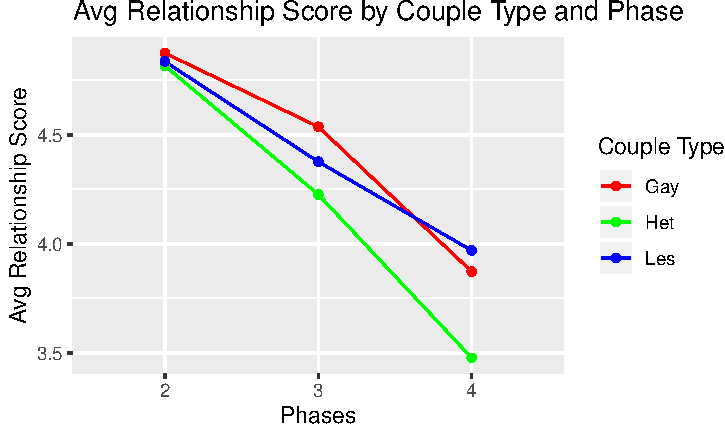
\includegraphics{final_paper_files/figure-latex/fig1-1.pdf}

For the maternal postnatal attachment scale, lesbian parents had a higher average across different phases. We also observed that during phase 2, LG parents experienced a rise in perceived attachment while heterosexual parents experienced a decrease.

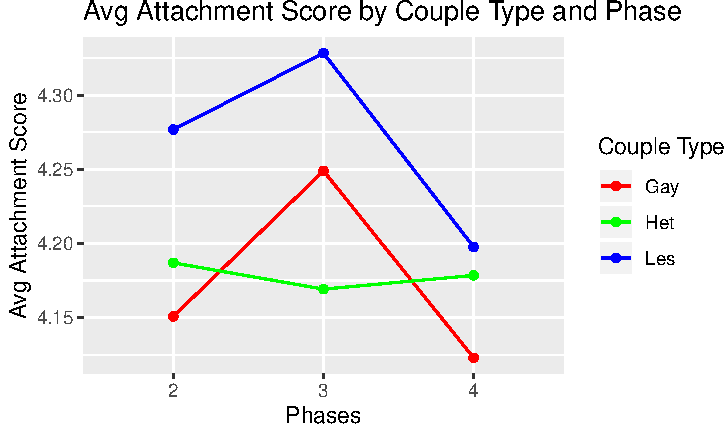
\includegraphics{final_paper_files/figure-latex/fig2-1.pdf}

For the anxiety scale, gay parents experience the most anxiety comparing with other groups. Both gay and heterosexual parents experienced an increase in anxiety from phase 3 to phase 4 while lesbian parents experienced a slight decrease.

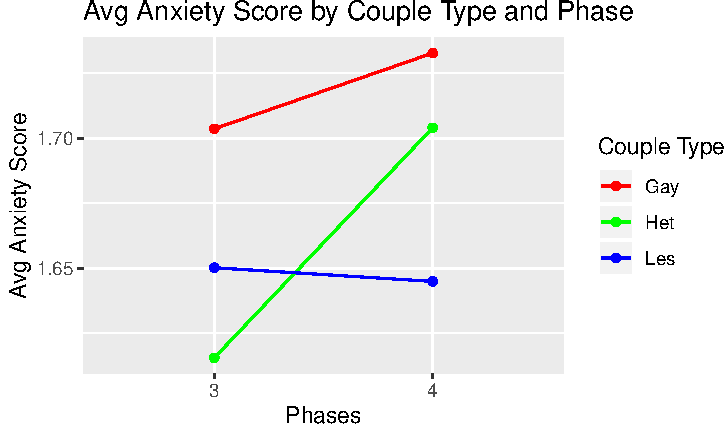
\includegraphics{final_paper_files/figure-latex/fig3-1.pdf}

For the depression scale, both heterosexual and lesbian parents experienced an increase in depression from phase 3 to phase 4 while gay parents experienced a decrease.

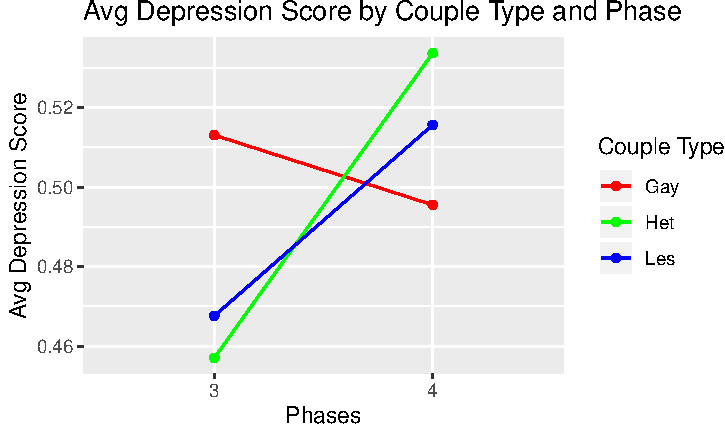
\includegraphics{final_paper_files/figure-latex/fig4-1.pdf}

By using an ANOVA test, we found that sexual orientation (homosexual or heterosexual) was a statistically significant predictor for relationship duration at phase 1. On average, homosexual couples in this study have been in a relationship for 1.76 years less than heterosexual couples.

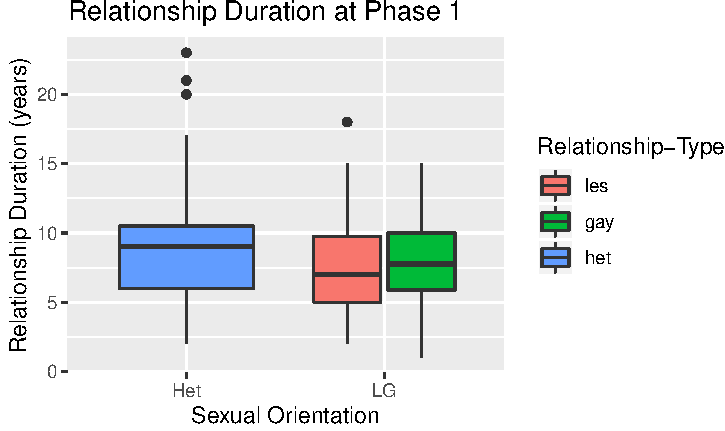
\includegraphics{final_paper_files/figure-latex/fig5-1.pdf}

\hypertarget{results}{%
\section{Results}\label{results}}

\begin{figure}

{\centering 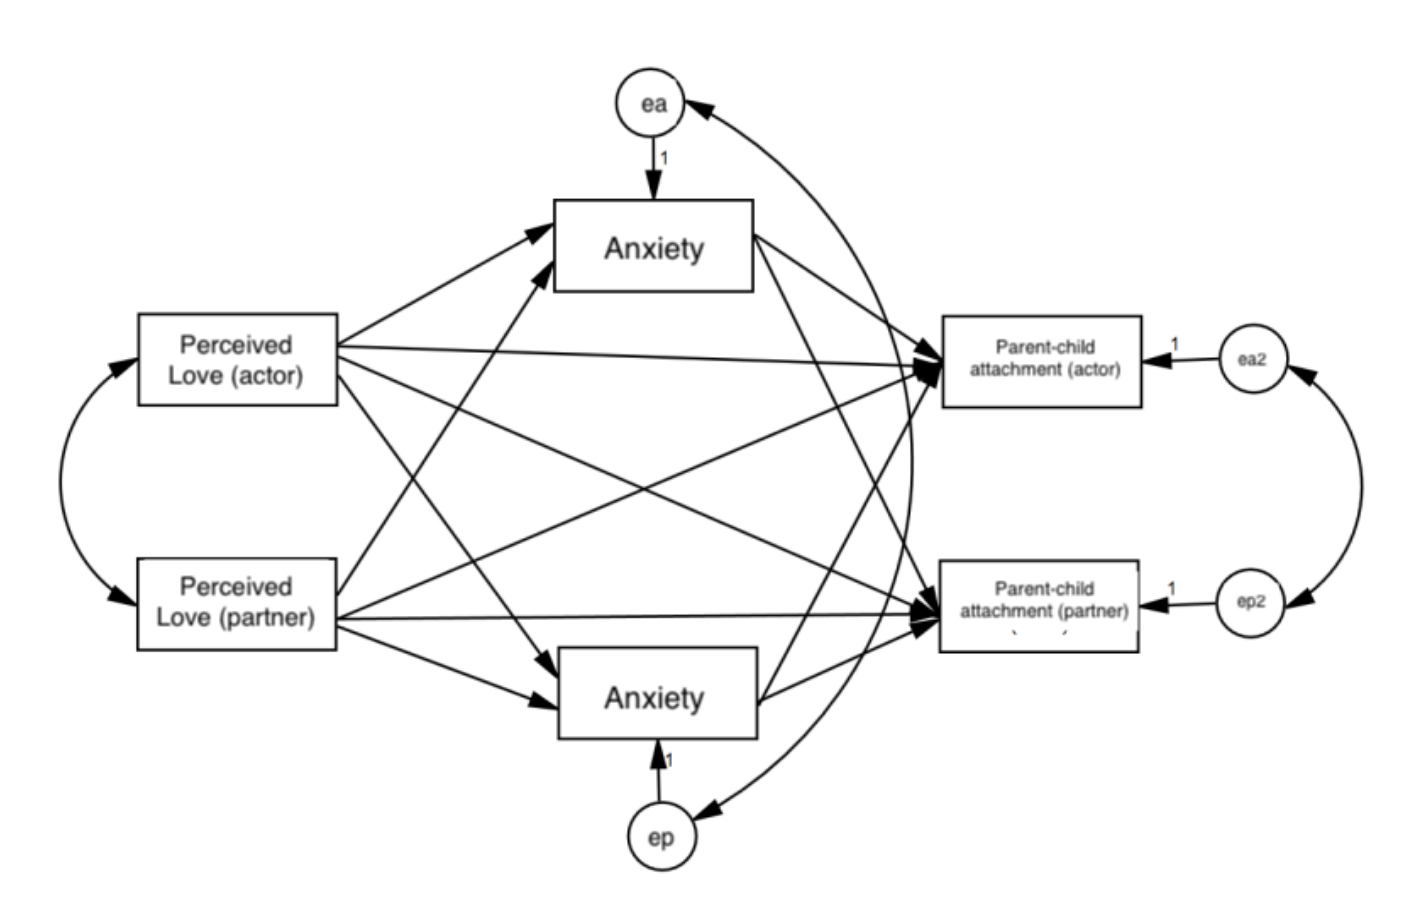
\includegraphics[width=500px]{figure1} 

}

\caption{Love and attachment mediated by anxiety}\label{fig:unnamed-chunk-3}
\end{figure}

\begin{figure}

{\centering 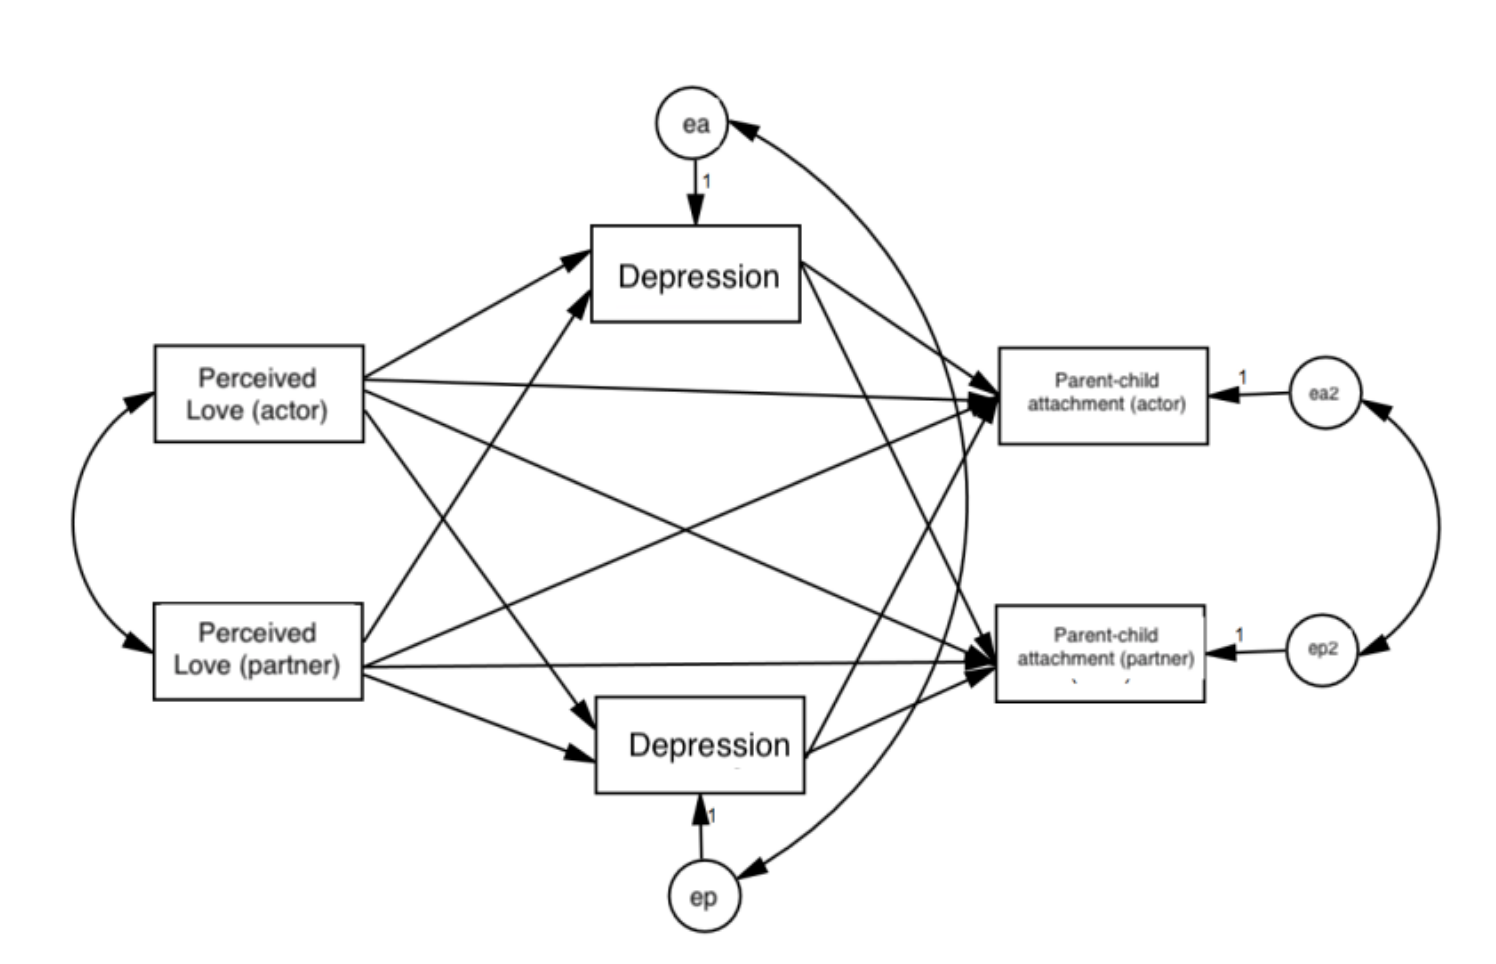
\includegraphics[width=500px]{figure2} 

}

\caption{Love and attachment mediated by depression}\label{fig:unnamed-chunk-4}
\end{figure}

\begin{table}[tbp]

\begin{center}
\begin{threeparttable}

\caption{\label{tab:unnamed-chunk-17}Predicting attachment with time and love}

\begin{tabular}{llllll}
\toprule
 & \multicolumn{1}{c}{Value} & \multicolumn{1}{c}{Std.Error} & \multicolumn{1}{c}{DF} & \multicolumn{1}{c}{t-value} & \multicolumn{1}{c}{p-value}\\
\midrule
(Intercept) & 3.45 & 0.20 & 572.00 & 17.45 & 0.00\\
time & 0.00 & 0.01 & 572.00 & -0.06 & 0.95\\
love\_A & 0.11 & 0.02 & 572.00 & 5.98 & 0.00\\
love\_P & -0.02 & 0.02 & 572.00 & -0.83 & 0.41\\
\bottomrule
\end{tabular}

\end{threeparttable}
\end{center}

\end{table}

\begin{table}[tbp]

\begin{center}
\begin{threeparttable}

\caption{\label{tab:unnamed-chunk-18}Predicting attachment with time and love and group*love interaction}

\begin{tabular}{llllll}
\toprule
 & \multicolumn{1}{c}{Value} & \multicolumn{1}{c}{Std.Error} & \multicolumn{1}{c}{DF} & \multicolumn{1}{c}{t-value} & \multicolumn{1}{c}{p-value}\\
\midrule
(Intercept) & 3.71 & 0.29 & 568.00 & 12.80 & 0.00\\
time & 0.00 & 0.01 & 568.00 & -0.08 & 0.93\\
love\_A & 0.06 & 0.03 & 568.00 & 1.97 & 0.05\\
groupgay & -0.75 & 0.50 & 138.00 & -1.48 & 0.14\\
grouples & -0.27 & 0.43 & 138.00 & -0.64 & 0.52\\
love\_P & 0.00 & 0.03 & 568.00 & 0.12 & 0.90\\
love\_A:groupgay & 0.12 & 0.05 & 568.00 & 2.58 & 0.01\\
love\_A:grouples & 0.07 & 0.05 & 568.00 & 1.47 & 0.14\\
groupgay:love\_P & -0.02 & 0.05 & 568.00 & -0.51 & 0.61\\
grouples:love\_P & -0.02 & 0.05 & 568.00 & -0.47 & 0.64\\
\bottomrule
\end{tabular}

\end{threeparttable}
\end{center}

\end{table}

\hypertarget{analysis-strategy}{%
\subsection{Analysis Strategy}\label{analysis-strategy}}

We hypothesized that the individuals' perception of love and their partner's perception of love in their relationship would affect the parent-child relationship positively, and associations would become stronger over time (hypothesis 1). We also hypothesized that the association between love and parent-child attachment would be different across family types (hypothesis 2). Furthermore, we hypothesized that depressive and anxiety symptoms play mediating roles in the association between love and attachment (hypotheses 3 and 4). We used multilevel modeling and the Actor-Partner Interdependence Model (APIM; Kenny, Kashy, and Cook (2006)) to test these hypotheses. The APIM simultaneously estimates the effect of one's perception of love in the relationship and the effect of the same variable but from the partner on parent-child attachment. Since our data was divided into three waves, the growth curve model was used. Given the characteristics of APIM and longitudinal dyadic data, we need to check for the intercept variance, slope variance, intercept covariance between dyad members, slope covariance, and slope-intercept covariance within-person and between.

In our first hypothesis, we used the following explanatory variables: 1) the actor's perception of love in the relationship, 2) partner's perception of love in the relationship, and 4) time. The response variable was the actor's attachment. In our second hypothesis, we added an interaction between love and actor-partner relationship type (lesbian, gay, or heterosexual). In our third and fourth hypotheses, we tested whether anxiety and depression of the actor could be potential mediators for the association between the love of the actor and the actor's perceived attachment. Figures 1 and 2 provide visual examples of what mediation looks like within an APIM. We used the Monte Carlo method (Tofighi \& MacKinnon, 2011) to assess mediation, which created confidence intervals for indirect effects.

\hypertarget{main-results}{%
\subsection{Main Results}\label{main-results}}

\hypertarget{hypothesis-1}{%
\subsubsection{Hypothesis 1:}\label{hypothesis-1}}

In our first model, the effect of the perception of love was statistically significant on the perceived parent-child attachment, such that the higher the perception of love, the more the person perceived that they were attached to their children (\emph{b} = 0.11, \emph{SE} = 0.019, \emph{p} \textless{} 0.001). Nevertheless, a person's partner's perception of love in their relationship did not show significant effects on themselves's or their partner's perceived parent-child attachment. We also found that time was not a statistically significant moderator for the correlation between love and attachment. In the association between love and attachment for a person at a time point, one did not predict the association between love and attachment for a person at the following time point. In the model the intercept variance was 0.05, intercept covariance was 0.02, and correlation between intercepts was 0.33. In regards to slope, the slope variance was \textless{}0.01, the slope covariance was \textless{}0.01, correlation between the slopes was 0.95, slope-intercept covariance (within a person) was \textless{}0.01, slope-intercept correlation (within a person) was 0.72, slope-intercept covariance (between persons) was 0.01, and slope-intercept correlation (between a person) was 0.89. Further details on the outcomes for the hypothesis test are provided in Table 1.

\hypertarget{hypothesis-2}{%
\subsubsection{Hypothesis 2:}\label{hypothesis-2}}

For our second hypothesis, we predicted that the relationship between the perception of love and parent-child attachment would be different across family types. Using the heterosexual couples as the reference group, we found the significant family type effects for the gay male couples (\emph{b} = 0.12, \emph{SE} = 0.05, \emph{p} = 0.01), but not for the lesbian couples (\emph{b} = 0.07, \emph{SE} = 0.05, \emph{p} = 0.14). The results partially supported our hypothesis that the difference in the association between perceived love and attachment existed across family types. Contrary to our prediction, we did not find the interaction of different family types on the correlation between love and parent-child attachment regarding time point statistically significant. In the model, the intercept variance was 0.05, intercept covariance was 0.02, and correlation between intercepts was 0.29. In regards to slope, the slope variance was \textless{}0.01, the slope covariance was \textless{}0.01, correlation between the slopes was 0.97, slope-intercept covariance (within a person) was \textless{}0.01, slope-intercept correlation (within a person) was 0.72, slope-intercept covariance (between persons) was 0.01, and slope-intercept correlation (between a person) was 0.87. Further details on the outcomes for the hypothesis test one are provided in Table 2.

\hypertarget{hypothesis-3}{%
\subsubsection{Hypothesis 3:}\label{hypothesis-3}}

To determine if anxiety mediates the relationship between perceived love in the parental relationship and parent-child relationship, a series of regression analyses were conducted. First, the love reported in the parental relationship (\emph{b} = 0.11, \emph{SE }= 0.04, \emph{p} \textless{} .001) significantly predicted parent-child attachment. Next, we found that the trait of anxiety was significantly predicted by an individual's perception of love in the relationship (\emph{b} = -0.11, \emph{SE} = 0.02, \emph{p} \textless{} 0.001). Finally, we found that an individual's perception of love (\emph{b} = 0.07, \emph{SE} = 0.02, \emph{p} \textless{} 0.01) and the trait of anxiety (\emph{b} = -0.33, \emph{SE} = 0.05, \emph{p} \textless{} 0.001) together significantly predicted parent-child attachment. The results revealed that anxiety negatively mediated the relationship between the perceived love in one's relationship and the perceived attachment to one's child. Finally, we used the Monte Carlo method (Tofighi \& MacKinnon, 2011) and found that the indirect effect of the mediation is statistically significant (CI ranges from 0.02 to 0.05).

\hypertarget{hypothesis-4}{%
\subsubsection{Hypothesis 4:}\label{hypothesis-4}}

In our fourth model, we found that there was a statistically significant mediation effect of depression in the link between love and attachment. From our previous model, we learned that there was a significant relationship between the actor's love and the actor's attachment. Then we tested and discovered that there was a statically significant actor effect of love on depression, such that the actor's depression level decreased with the increase of their own perceived love (\emph{b} = -0.10, \emph{SE} = 0.02, \emph{p} \textless{} 0.001). We further tested the direct effect of actor's love and their depression on attachment in a full model and found that both the actor effect of love (\emph{b} = 0.07, \emph{SE} = 0.02, \emph{p} \textless{} 0.001) and depression (\emph{b} = -0.27, \emph{SE} = 0.05, \emph{p} \textless{} 0.001) were statistically related to attachment. This mediation was such that a person who was high in perceived love had a lower level of depression, while a higher level of depression also negatively influence their perceived parent-child attachment. Finally, we used the Monte Carlo method (Tofighi \& MacKinnon, 2011) and found that the indirect effect of the mediation is statistically significant (CI ranges from 0.02 to 0.05).

In the full model, we also found time as a statistically significant predictor for the association between depression and love attachment (\emph{b} = -0.07, \emph{SE} = 0.03, \emph{p} = 0.04). However, we deduced the significance to be inconclusive since we did not find significant associations between time and either attachment or love.

\hypertarget{discussion}{%
\section{Discussion}\label{discussion}}

We hypothesized that an individual's perception of love in their relationship and their partner's perception of love would be associated with the parent-child attachment, and the association would be moderated by time. The model revealed that only the actor's perception of love was positively associated with the attachment. This result aligns with the past findings that children's attachment security is associated with love (Obeldobel \& Kerns, 2019). Contrary to our prediction, we did not find any significant time effect in the association. Sroufe, Egeland, Carlson, and Collins (2009) has examined attachment over several years and reported stability in the attachment, which supports these findings.

In our second hypothesis, we assumed that the relationship between the perception of love and parent's perceived attachment to their children would be different across family types, controlled by time. We found that the association between perception of love and parent's perceived attachment was stronger for gay male couples but not for lesbian couples in comparison to heterosexual couples. The results partially supported our hypothesis that the association would change across family types. McConnachie et al. (2019) examined attachment security of children in gay father families, lesbian mother families, and heterosexual parent families. They found that children in gay father families showed significantly higher levels of secure-autonomous attachment than children in heterosexual parent families. Our findings added evidence in the investigation of the differences in the parent-children attachment between gay father families and heterosexual families and further indicated that the differences exist in the association between parental perceived love and parent-child attachment.

In our third hypothesis, we proposed that anxiety can serve as a mediating role in the association between love and attachment. We found support for our hypothesis that an anxious personality negatively mediated the correlation between love and attachment. Past findings establish the links between anxiety and parental relationship and children's attachment. For example, Stevenson-Hinde et al. (2011) found that poor dyadic adjustment is associated with higher levels of anxiety, and maternal anxiety is negatively correlated with the ratings of children's attachment. Our findings support the hypothesis that anxiety mediates parental relationships and parent-child attachment.

Our last hypothesis was that depressive symptoms would mediate the association between perceived love and attachment. Our results indicated that depressive symptoms negatively mediated the relationship between one's perceived love within the relationship and one's attachment to their child. Previous studies have found that depression has associations with parental relationships and parent-child attachment (Santona et al., 2015; Stevenson-Hinde et al., 2011), and our findings support these ideas by revealing that depression mediates the relationship between love (within the couple) and parent-child attachment.

The current study has the strength of including diverse family structures in terms of couple types by comparing different gay, lesbian, and heterosexual couples. Furthermore, the longitudinal data allowed us to explore the stability of the association between perceived love in the dyadic relationship and parent-child attachment. As established studies have mostly focused on the children's attachment to their biological parents in heterosexual parent families, our study adds insight on different measures and samples by exploring gay and lesbian parents' attachment to their children in adoptive families.

Our study had several limitations. One of them is incomplete data for variables throughout phases. Data on anxiety and depression was missing for Phase 2, so we were limited to test hypotheses 3 and 4 only for Phase 3 and Phase 4. Another limitation of this study is low internal consistency for perceived attachment in Phase 2, which indicated low reliability of the measurement. We speculated that the low across items reliability of the dependent variable might be a potential explanation for the non-significant time effect. In addition, we did not exclude alternative explanations. For example, some studies revealed that gay families might tend to present their families as high functioning. Due to the difficulties in adopting children and the stigma they experienced from the outside world, they may want to \enquote{fake good} in self-reported measures (Bellack, Hersen, \& Kazdin, 2012). As our study supported a stronger association between perceived love and attachment for gay male couples, the differences could be due to the failure of measuring genuine relationships in gay father families.

In our current study, we selected love as a subscale because, within the original relationship questionnaire, only love showed an actor effect on perceived parent-child attachment. In future studies, we would like to examine other subscales and explore their relationship with perceived attachment. Additionally, researchers might also want to replicate our study by using different measures. For example, as our study examined the mediator role of anxiety as a personality, it may be interesting to explore the role of anxiety as a mental health condition in the relationship between perceived love and attachment. As it is difficult to \enquote{fake good} with observational measures (Kerig \& Lindahl, 2000), future studies could use different study designs to compare the differences among family types.

Our results align and reinforce the current findings of the impacts of parental relationship quality, parents' mental health conditions, and family types on the parent-child relationship. Specifically, our results provided insights into the dynamics of adoptive families by including not only heterosexual parents but also lesbian and gay parents. The current study also has practical implications. Children in foster families are vulnerable to delinquent behaviors and misconduct. As the parent-child relationship is one of the crucial predictors for antisocial behaviors of children in the future, our findings can aid in the development of prevention and intervention programs for adoptive families to improve relationships within the family and further, to foster better life outcomes for adopted children.

\newpage

\hypertarget{references}{%
\section{References}\label{references}}

\begingroup
\setlength{\parindent}{-0.5in}
\setlength{\leftskip}{0.5in}

\hypertarget{refs}{}
\leavevmode\hypertarget{ref-amato1996prospective}{}%
Amato, P. R., \& Booth, A. (1996). A prospective study of divorce and parent-child relationships. \emph{Journal of Marriage and the Family}, 356--365.

\leavevmode\hypertarget{ref-bellack2012international}{}%
Bellack, A. S., Hersen, M., \& Kazdin, A. E. (2012). \emph{International handbook of behavior modification and therapy}. Springer Science \& Business Media.

\leavevmode\hypertarget{ref-braiker1979conflict}{}%
Braiker, H. B., \& Kelley, H. H. (1979). Conflict in the development of close relationships. \emph{Social Exchange in Developing Relationships}, \emph{135}, 168.

\leavevmode\hypertarget{ref-brodzinsky2014children}{}%
Brodzinsky, D. M., Schechter, D., \& Brodzinsky, A. B. (2014). Children's knowledge of adoption: Developmental changes and implications for adjustment. In \emph{Thinking about the family} (pp. 225--252). Psychology Press.

\leavevmode\hypertarget{ref-condon1997correlates}{}%
Condon, J. T., \& Corkindale, C. (1997). The correlates of antenatal attachment in pregnant women. \emph{British Journal of Medical Psychology}, \emph{70}(4), 359--372.

\leavevmode\hypertarget{ref-cummings1994children}{}%
Cummings, E. M., \& Davies, P. (1994). \emph{Children and marital conflict: The impact of family dispute and resolution.} Guilford Press.

\leavevmode\hypertarget{ref-study3}{}%
Cyr, M., Pasalich, D. S., McMahon, R. J., \& Spieker, S. J. (2014). The longitudinal link between parenting and child aggression: The moderating effect of attachment security. \emph{Child Psychiatry \& Human Development}, \emph{45}(5), 555--564.

\leavevmode\hypertarget{ref-dickstein2009maternal}{}%
Dickstein, S., Seifer, R., \& Albus, K. E. (2009). Maternal adult attachment representations across relationship domains and infant outcomes: The importance of family and couple functioning. \emph{Attachment \& Human Development}, \emph{11}(1), 5--27.

\leavevmode\hypertarget{ref-fergusson2005show}{}%
Fergusson, D. M., John Horwood, L., \& Ridder, E. M. (2005). Show me the child at seven: The consequences of conduct problems in childhood for psychosocial functioning in adulthood. \emph{Journal of Child Psychology and Psychiatry}, \emph{46}(8), 837--849.

\leavevmode\hypertarget{ref-gao2019understanding}{}%
Gao, M. M., \& Cummings, E. M. (2019). Understanding parent--child relationship as a developmental process: Fluctuations across days and changes over years. \emph{Developmental Psychology}.

\leavevmode\hypertarget{ref-ghunney2011beyond}{}%
Ghunney, A. K.-K. (2011). Beyond race and ethnicity: Predictors of maternal depressive symptoms across the transition to parenthood.

\leavevmode\hypertarget{ref-goldberg2009perceived}{}%
Goldberg, A. E., \& Smith, J. Z. (2009). Perceived parenting skill across the transition to adoptive parenthood among lesbian, gay, and heterosexual couples. \emph{Journal of Family Psychology}, \emph{23}(6), 861.

\leavevmode\hypertarget{ref-golombok2014adoptive}{}%
Golombok, S., Mellish, L., Jennings, S., Casey, P., Tasker, F., \& Lamb, M. E. (2014). Adoptive gay father families: Parent--child relationships and children's psychological adjustment. \emph{Child Development}, \emph{85}(2), 456--468.

\leavevmode\hypertarget{ref-apim}{}%
Kenny, D. A., Kashy, D. A., \& Cook, W. L. (2006). \emph{Dyadic data analysis}. Guilford press.

\leavevmode\hypertarget{ref-kerig1993marital}{}%
Kerig, P. K., Cowan, P. A., \& Cowan, C. P. (1993). Marital quality and gender differences in parent-child interaction. \emph{Developmental Psychology}, \emph{29}(6), 931.

\leavevmode\hypertarget{ref-kerig2000introduction}{}%
Kerig, P. K., \& Lindahl, K. M. (2000). Introduction and overview: Conceptual issues in family observational research. In \emph{Family observational coding systems} (pp. 17--38). Psychology Press.

\leavevmode\hypertarget{ref-klausli2011exploring}{}%
Klausli, J. F., \& Tresch Owen, M. (2011). Exploring actor and partner effects in associations between marriage and parenting for mothers and fathers. \emph{Parenting}, \emph{11}(4), 264--279.

\leavevmode\hypertarget{ref-laurent2008prospective}{}%
Laurent, H. K., Kim, H. K., \& Capaldi, D. M. (2008). Prospective effects of interparental conflict on child attachment security and the moderating role of parents' romantic attachment. \emph{Journal of Family Psychology}, \emph{22}(3), 377.

\leavevmode\hypertarget{ref-levy1991transition}{}%
Levy-Shiff, R., Goldshmidt, I., \& Har-Even, D. (1991). Transition to parenthood in adoptive families. \emph{Developmental Psychology}, \emph{27}(1), 131.

\leavevmode\hypertarget{ref-mcconnachie2019father}{}%
McConnachie, A. L., Ayed, N., Jadva, V., Lamb, M., Tasker, F., \& Golombok, S. (2019). Father-child attachment in adoptive gay father families. \emph{Attachment \& Human Development}, 1--14.

\leavevmode\hypertarget{ref-obeldobel2019attachment}{}%
Obeldobel, C. A., \& Kerns, K. A. (2019). Attachment security is associated with the experience of specific positive emotions in middle childhood. \emph{Attachment \& Human Development}, 1--13.

\leavevmode\hypertarget{ref-reef2011developmental}{}%
Reef, J., Diamantopoulou, S., Meurs, I. van, Verhulst, F. C., \& Ende, J. van der. (2011). Developmental trajectories of child to adolescent externalizing behavior and adult dsm-iv disorder: Results of a 24-year longitudinal study. \emph{Social Psychiatry and Psychiatric Epidemiology}, \emph{46}(12), 1233--1241.

\leavevmode\hypertarget{ref-santona2015maternal}{}%
Santona, A., Tagini, A., Sarracino, D., De Carli, P., Pace, C. S., Parolin, L., \& Terrone, G. (2015). Maternal depression and attachment: The evaluation of mother--child interactions during feeding practice. \emph{Frontiers in Psychology}, \emph{6}, 1235.

\leavevmode\hypertarget{ref-singer1985mother}{}%
Singer, L. M., Brodzinsky, D. M., Ramsay, D., Steir, M., \& Waters, E. (1985). Mother-infant attachment in adoptive families. \emph{Child Development}, 1543--1551.

\leavevmode\hypertarget{ref-spielberger1983state}{}%
Spielberger, C. D. (1983). State-trait anxiety inventory for adults.

\leavevmode\hypertarget{ref-sroufe2009development}{}%
Sroufe, L. A., Egeland, B., Carlson, E. A., \& Collins, W. A. (2009). \emph{The development of the person: The minnesota study of risk and adaptation from birth to adulthood}. Guilford Press.

\leavevmode\hypertarget{ref-stevenson2007anxiety}{}%
Stevenson-Hinde, J., Curley, J. P., Chicot, R., \& Jóhannsson, C. (2007). Anxiety within families: Interrelations, consistency, and change. \emph{Family Process}, \emph{46}(4), 543--556.

\leavevmode\hypertarget{ref-stevenson2011maternal}{}%
Stevenson-Hinde, J., Shouldice, A., \& Chicot, R. (2011). Maternal anxiety, behavioral inhibition, and attachment. \emph{Attachment \& Human Development}, \emph{13}(3), 199--215.

\leavevmode\hypertarget{ref-monte}{}%
Tofighi, D., \& MacKinnon, D. P. (2011). RMediation: An r package for mediation analysis confidence intervals. \emph{Behavior Research Methods}, \emph{43}(3), 692--700.

\leavevmode\hypertarget{ref-umberson2006you}{}%
Umberson, D., Williams, K., Powers, D. A., Liu, H., \& Needham, B. (2006). You make me sick: Marital quality and health over the life course. \emph{Journal of Health and Social Behavior}, \emph{47}(1), 1--16.

\leavevmode\hypertarget{ref-van2005dynamic}{}%
Van Geert, P. L., \& Lichtwarck-Aschoff, A. (2005). A dynamic systems approach to family assessment. \emph{European Journal of Psychological Assessment}, \emph{21}(4), 240--248.

\leavevmode\hypertarget{ref-van2006emanuel}{}%
Van IJzendoorn, M. H., \& Juffer, F. (2006). The emanuel miller memorial lecture 2006: Adoption as intervention. Meta-analytic evidence for massive catch-up and plasticity in physical, socio-emotional, and cognitive development. \emph{Journal of Child Psychology and Psychiatry}, \emph{47}(12), 1228--1245.

\leavevmode\hypertarget{ref-whisman2012intimate}{}%
Whisman, M. A., \& Baucom, D. H. (2012). Intimate relationships and psychopathology. \emph{Clinical Child and Family Psychology Review}, \emph{15}(1), 4--13.

\endgroup


\end{document}
